\section{Resultados}
Los resultados han sido divididos en dos partes: bibliométricos e ingeniería. 

\subsection{Resultados bibliometricos}
Luego del proceso de identificación de documentos científicos especificado en la figura 1, los artículos fueron ordenados según su año de publicación. En la figura 2, se puede identificar cómo en los últimos años el 2025 tuvo la mayor cantidad de producción científica con 10 artículos publicados, lo cual a su vez representa el 37\% con respecto al total.

\begin{figure}[H]
\begin{center}
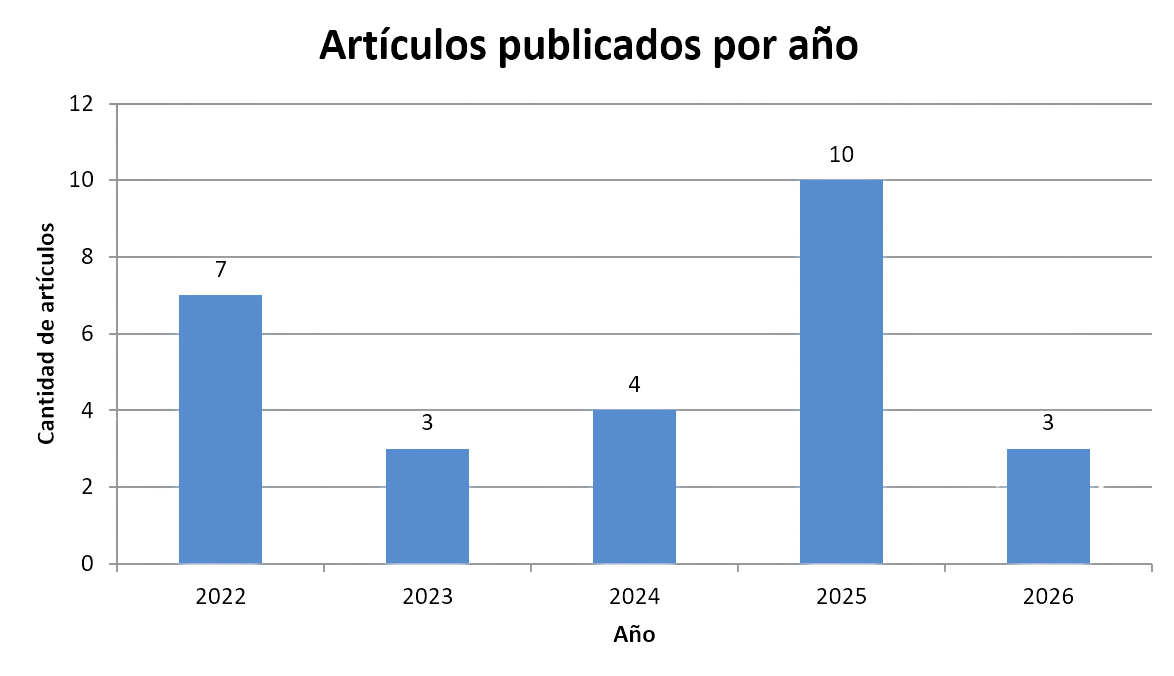
\includegraphics[width=8cm]{figures/fig3.png}
\end{center}
\caption{Artículos científicos por año}
\label{figura3}
\end{figure}


\begin{figure}[H]
\begin{center}
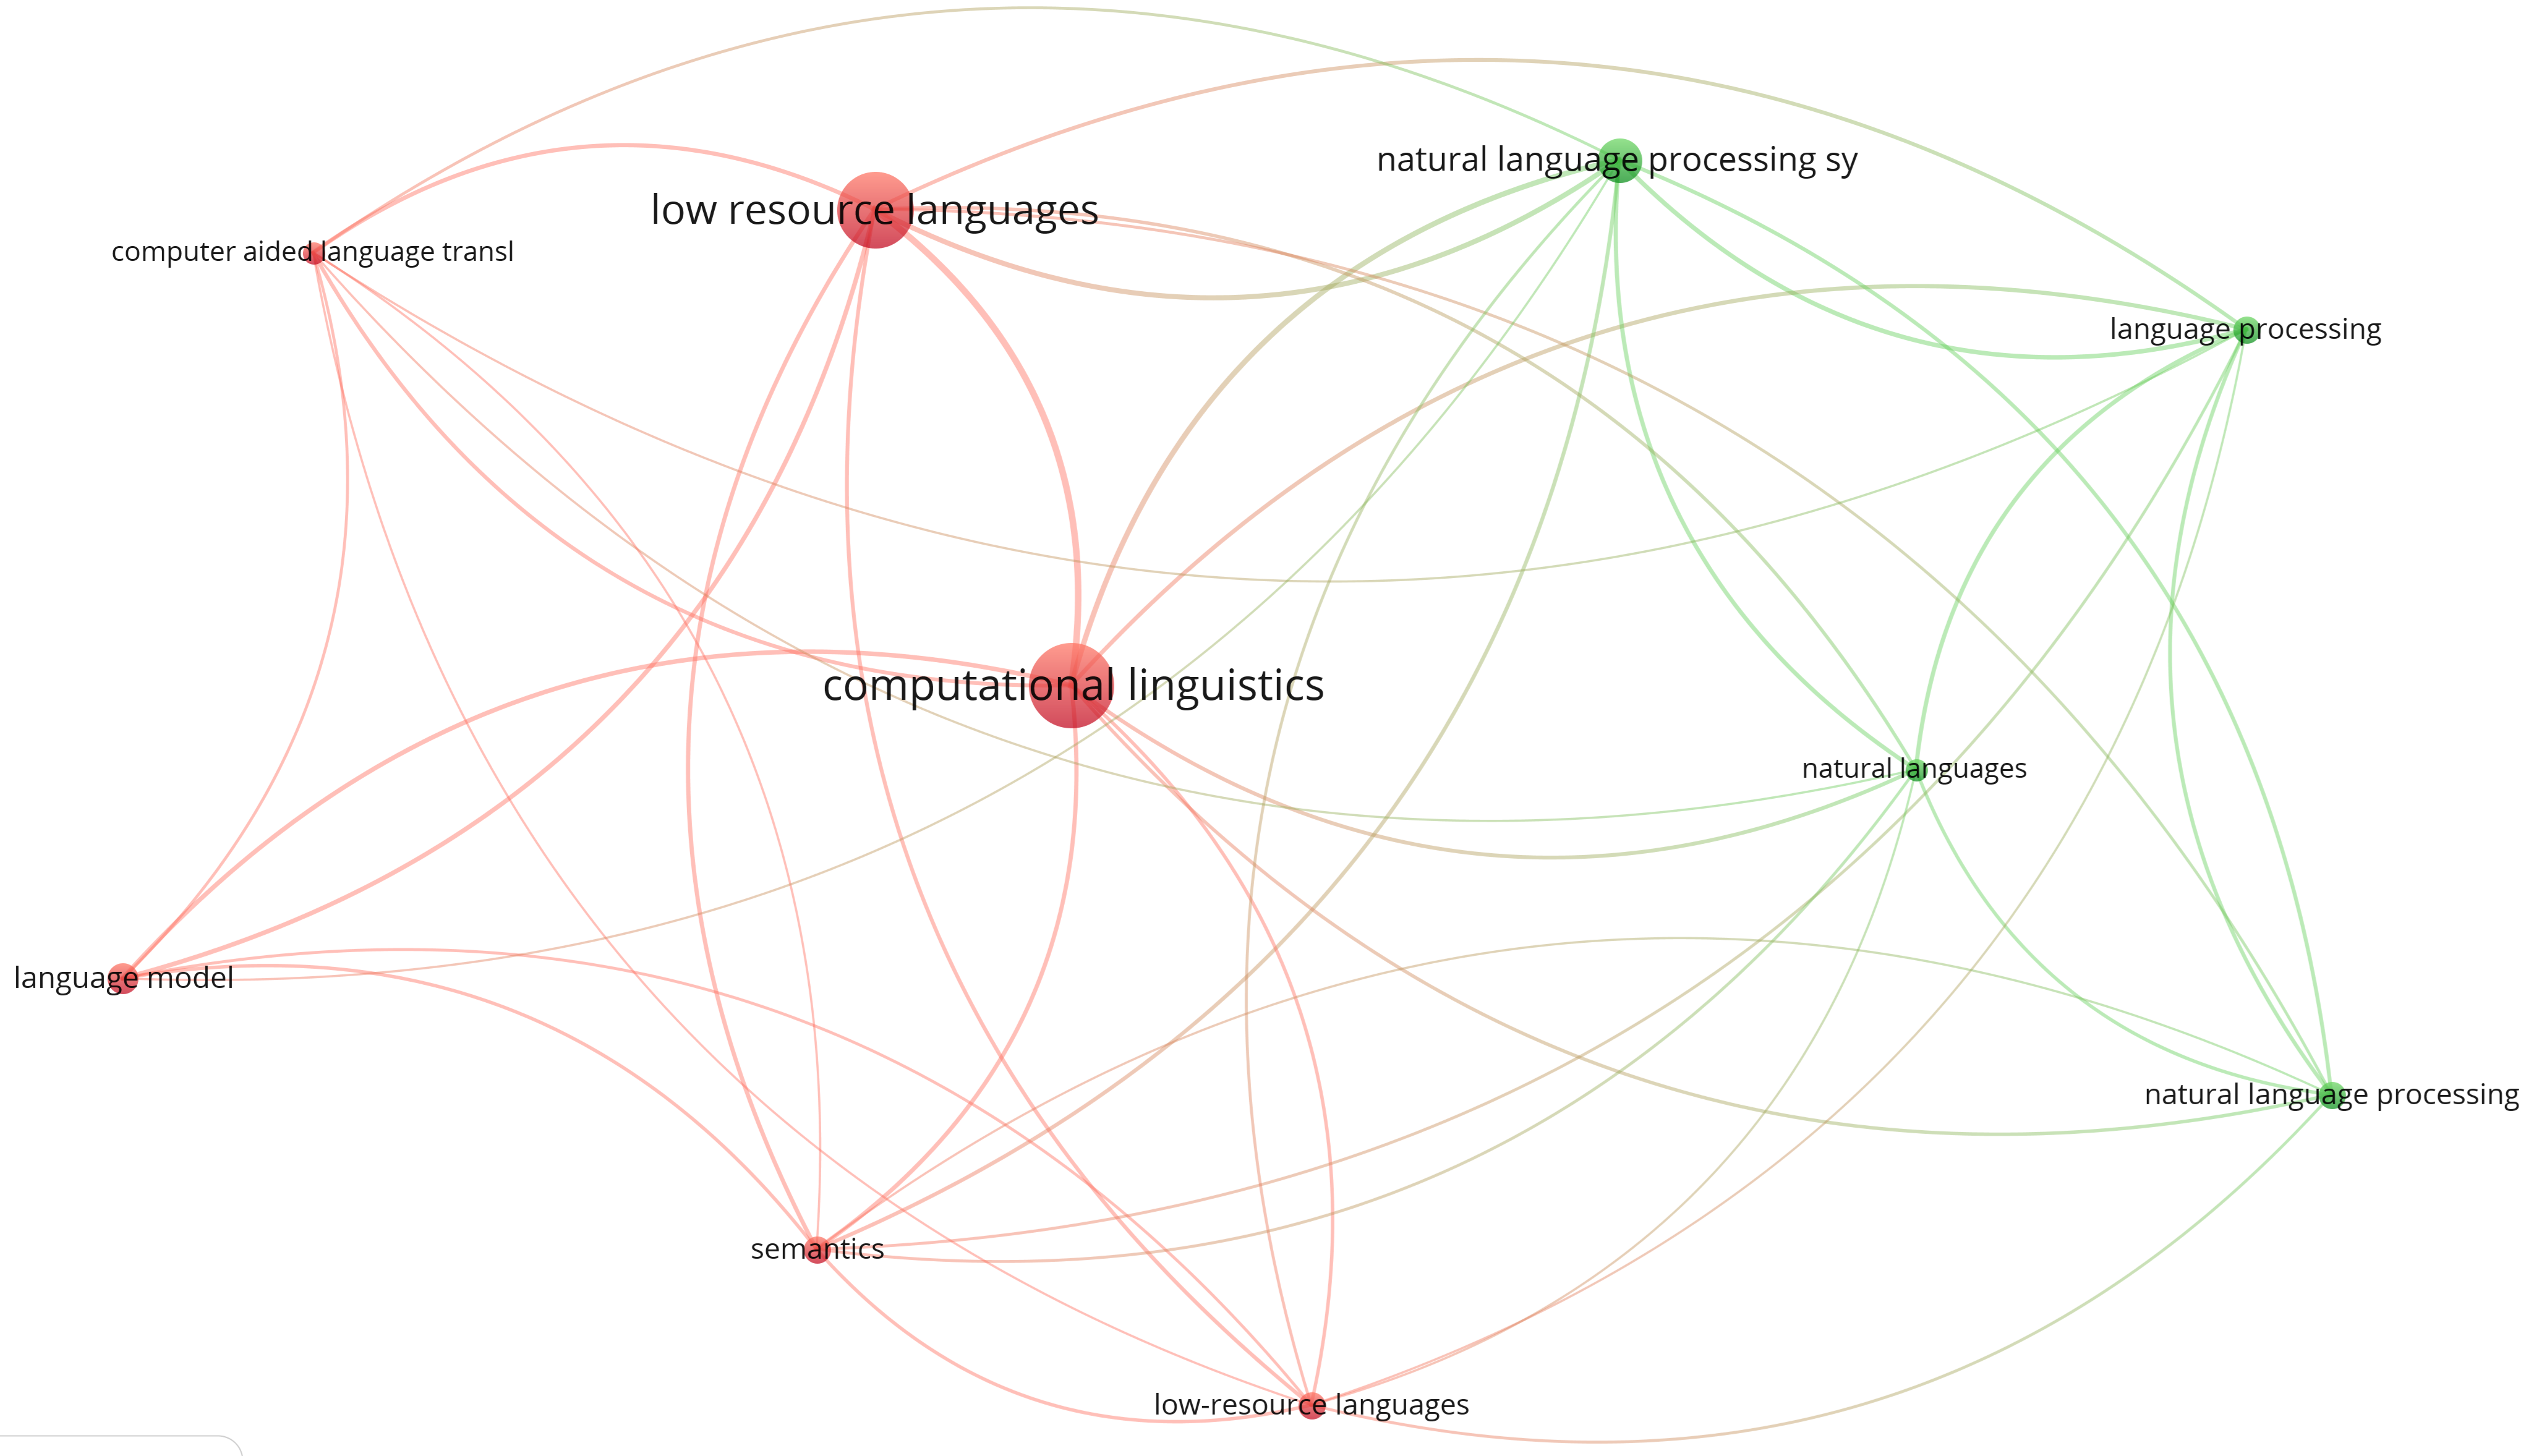
\includegraphics[width=8cm]{figures/fig4.png}
\end{center}
\caption{Red de coocurrencia de palabras clave}
\label{figura4}
\end{figure}

La figura 3 presenta la red de coocurrencia, la cual evidencia cómo se relacionan las palabras clave dentro de los artículos analizados. Se estableció un umbral de un mínimo de 5 ocurrencias por término, de las cuales solo 10 de 256 cumplieron este criterio. Asimismo, los conceptos con mayor centralidad son \textit{computational linguistics} con 19 ocurrencias, y \textit{low resource languages} con 17 ocurrencias; la proximidad entre ambos nodos y la mayor densidad de enlace, reflejan la alta frecuencia de aparición conjunta de ambas palabras clave. Por otro lado, es posible identificar por los colores rojo y verde la división entre dos grupos: el primero (rojo), agrupa las palabras orientadas a modelos, semántica y lenguajes de bajos recursos; mientras que el segundo (verde), destaca por su relación con el Procesamiento de Lenguaje Natural (NLP).

\begin{figure}[H]
\begin{center}
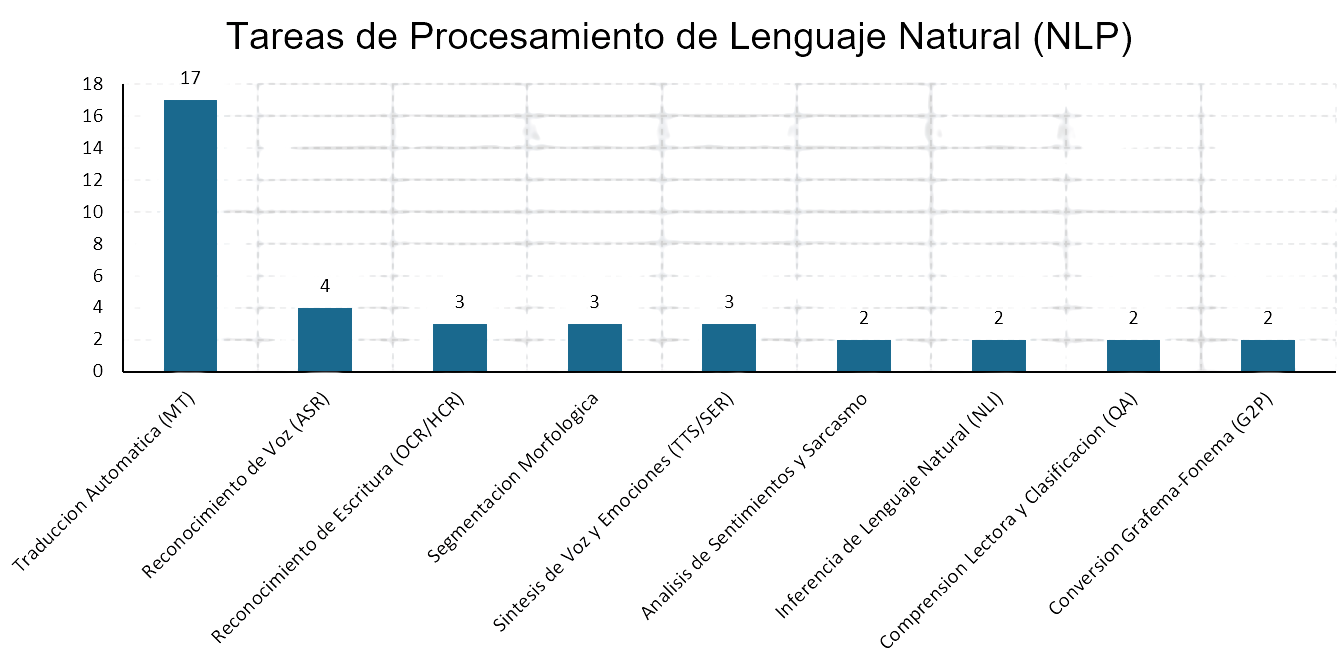
\includegraphics[width=8cm]{figures/fig5.png}
\end{center}
\caption{Tareas de Procesamiento de Lenguaje Natural (NLP)}
\label{figura5}
\end{figure}

\begin{figure}[H]
\begin{center}
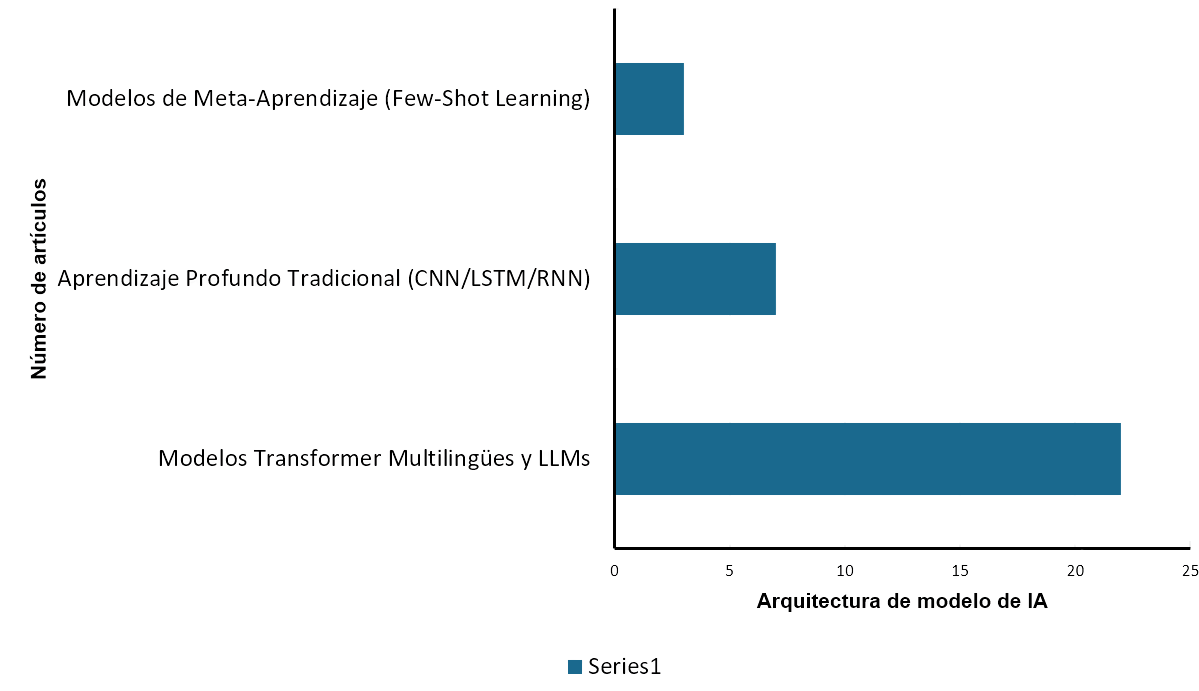
\includegraphics[width=8cm]{figures/fig6.png}
\end{center}
\caption{Arquitecturas y Modelos de Inteligencia Artificial}
\label{figura6}
\end{figure}

\begin{figure}[H]
\begin{center}
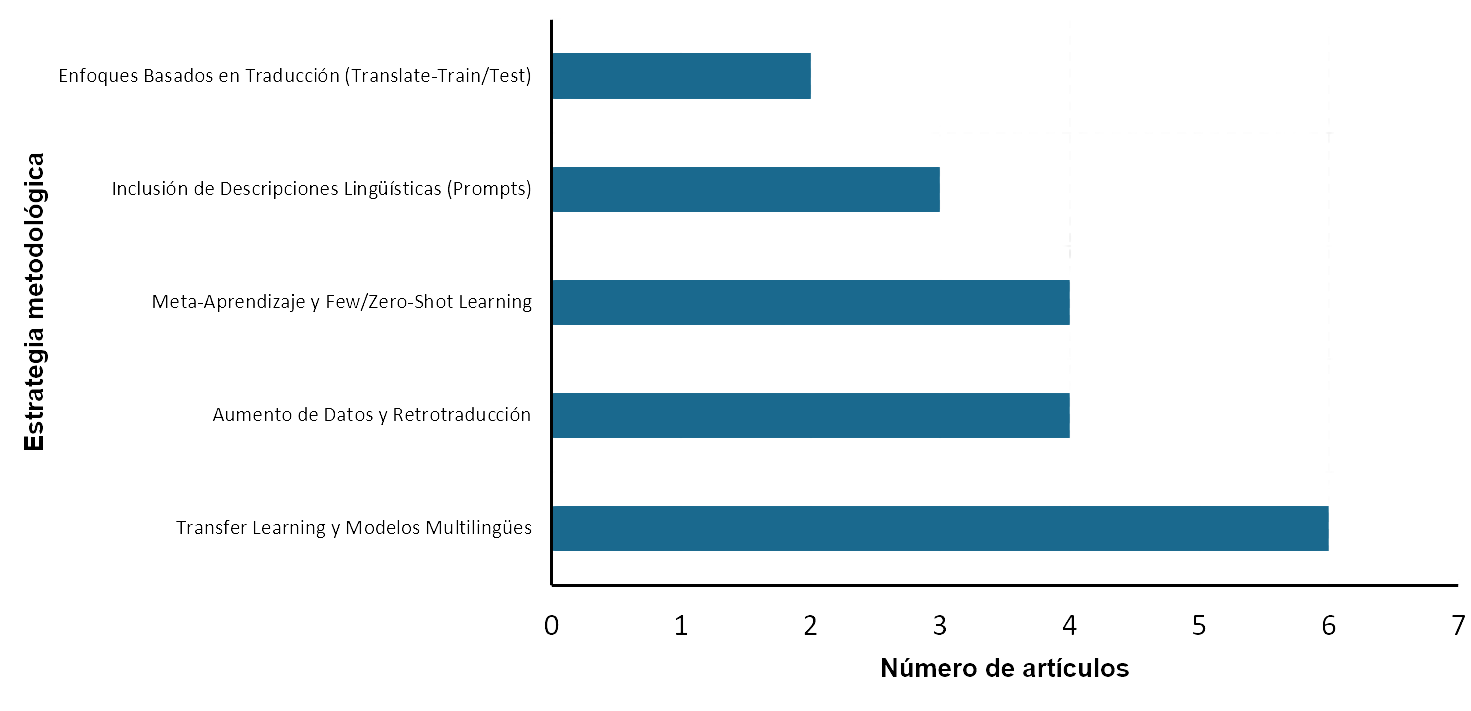
\includegraphics[width=8cm]{figures/fig7.png}
\end{center}
\caption{Estrategias para Mitigar la Escasez de Datos}
\label{figura7}
\end{figure}


\subsection{Resultados de ingeniería}
[Por completar]

% Estos dos apartados suelen aparecer juntos en muchos trabajos. No se deben confundiCoocurrenciacr esta discusión o análisis con la obtención de conclusiones, algo que depende tanto de los resultados y de su análisis como del marco teórico y de los objetivos.

% El pseudocódigo de los algoritmos debe ser presentado según indica el ejemplo del algortimo

% \begin{algorithm}[H]
% \label{algo1}
% \SetAlgoLined
% \text{\textbf{Entrada:}} \text{Caso estudio}\\
% \text{\textbf{Salida:}} \text{Global solución}\\
% \KwResult{Escribir aquí el resultado }
%  initialización\;
%  \While{While condicion}{
%   instructions\;
%   \eIf{condición}{
%    instrucciones1\;
%    instrucciones2\;
%    }{
%    instrucciones3\;
%   }
%  }
%  \caption{Como escribir algoritmos}
% \end{algorithm}





%========================================================
